\documentclass[11pt, hidelinks, letterpaper, obeyspaces]{article}
\usepackage[english]{babel}
\usepackage[T1]{fontenc}
\usepackage{fancyhdr}
\usepackage{framed}
\usepackage{titling}
\usepackage{extramarks}
\usepackage{lmodern}
\usepackage{hyperref}
\usepackage{bookmark}
\usepackage{titlesec}
% \usepackage{ragged2e}
\usepackage{csquotes}
\usepackage{lastpage}
\usepackage{minted}
% \usepackage{draftwatermark}
\usepackage{pdfpages}
\usepackage[framemethod=TikZ]{mdframed}
\usetikzlibrary{shadows}

% \SetWatermarkText{\textbf{DRAFT}}
% \SetWatermarkScale{1.2}
% \SetWatermarkColor[gray]{0.9}

\newcommand{\documentTitle}{Database Search Utility Requirments and Technical
  Notes}
\newcommand{\documentName}{\documentTitle}
\newcommand{\clientName}{Central Coast Climate Collaborative}
\newcommand{\clientWebsite}{\url{https://www.centralcoastclimate.org/}}
\newcommand{\authorName}{Dominic Gaiero}
\newcommand{\authorEmail}{\href{mailto:dgaiero@calpoly.edu}
  {\url{dgaiero@calpoly.edu}}}
\newcommand{\revNumber}{\texttt{0.1}}
\author{\authorName}
\title{\documentTitle\ - \clientName}

\hypersetup{
    pdftitle={\documentTitle\ - \clientName},
    pdfsubject={\documentName},
    pdfauthor={\authorName}
}
\tikzset{every shadow/.style={opacity=1}}
\newmdenv[shadow=true,shadowcolor=black,font=\sffamily, 
          align=right, leftmargin=10pt]{shadowbox}

\topmargin=-0.45in
\evensidemargin=0in
\oddsidemargin=0in
\textwidth=6.5in
\textheight=9.0in
\headsep=0.25in
\setlength{\headheight}{26pt}

\pagestyle{fancy}
\lhead{\textbf{\clientName}\\\clientWebsite}
\rhead{\documentTitle\\\authorName}
\lfoot{Rev: \revNumber}
\cfoot{}
\rfoot{\thepage}

\renewcommand{\headrulewidth}{2pt}
\renewcommand{\footrulewidth}{1pt}
% \renewcommand*\ttdefault{lmvtt} % for Latin Modern Mono Proportional
% \renewcommand{\familydefault}{\ttdefault}
\renewcommand{\familydefault}{\sfdefault}

\renewenvironment{leftbar}{%
  \def\FrameCommand{\vrule width 0.8pt \hspace{10pt}}%
  \MakeFramed {\advance\hsize-\width \FrameRestore}}%
 {\endMakeFramed}

\titleformat{\chapter}[display]
  {\normalfont\bfseries}{}{0pt}{\Huge}

\setlength{\parindent}{4em}
\setlength{\parskip}{0.5em}

\begin{document}
\begin{titlepage}
    \setlength{\parindent}{0pt}
    \setlength{\parskip}{0pt}
    \vspace*{\stretch{1}}
    \rule{\linewidth}{2pt}
    \begin{flushleft}
    \Huge \textbf{\documentTitle} \\
    \Large \textit{\href{https://www.centralcoastclimate.org}
      {\url{\clientName}}} \\[14pt]
    \Large \authorName\\
    \normalsize \authorEmail
    \end{flushleft}
    \rule{\linewidth}{1pt}
    Revision: \revNumber
    \vspace*{\stretch{2}}
\end{titlepage}
\newpage
\tableofcontents\thispagestyle{fancy}

\begin{shadowbox}
  \large \textbf{Product Delivery Notes}\\
  \normalsize
   An MVP version of this web application will be available by mid-July 2019.
\end{shadowbox}

\newpage
\section{Executive Overview}\thispagestyle{fancy}
This web application will serve as a lookup database for institution personal,
faculty and collaborators to use for information request.
This web application shall reside on a website open to the public and provide
a view to allow easy searching of database objects.
% \section{User Stories}\thispagestyle{fancy}
% \subsection{Institution}
The first type of user to look at is an institution. An institution may wish to
search for another institution offering 
\section{Development Stack}\thispagestyle{fancy}
For a complete list of all expected python (core) dependencies for this project,
please reference appendix section~\ref{sec:requirements.txt}
\par This web application will utilize the Django web framework. For front-end
development, React will be utilized.
% \section{Development Practices}\thispagestyle{fancy}
\section{Security Considerations}\thispagestyle{fancy}
\begin{itemize}
  \item This web application will be open on the Internet to anyone  who wishes
  to access this website. All non-administrative pages of this web application
  will not be accessed controlled.
  \item Administrative sections of this web application will be accessed
  controlled through the built in mechanisms provided via the Django web
  framework.
\end{itemize}
\section{Production Requirements}\thispagestyle{fancy}
\subsection{Minimum Server Hardware Requirements}
The server hosting this web application should have:
\begin{enumerate}
  \item 512 MB RAM
  \item 1 CPU Core
  \item 2 GB free HDD space (allocated size mostly for database.)
  \begin{enumerate}
    \item If the database if hosted on another node, then this requirement can
    be far smaller (500 MB).
  \end{enumerate}
  \item Appropriate bandwidth
  \begin{enumerate}
    \item For a low-usage web application such as the one being built, the
    bandwidth that is available from the \clientName's website will be
    appropriate.
  \end{enumerate}
\end{enumerate}
\subsection{Server Software Requirements}
Development of this web application shall be supported on both Nginx and Apache.
The database for this web application is supported on both PostgreSQL and MySQL.
The choice to support both Apache and MySQL is due to the fact that the
preferred deployment of WordPress uses both of these technologies.
\begin{leftbar}
  \noindent\textbf{NOTE: }The preferred method for configuration is on
  Nginx with PostgreSQL.
\end{leftbar}
\subsubsection{Baseline Considerations}
\begin{itemize}
  \item The server, for any configuration will require \verb!sudo! mode privilege
    escalation to implement the setup for a production environment.
  \item The server will also require Python3 installed with access to install other
    python packages (those specified inside of the
    \hyperref[sec:requirements.txt]{\url{requirements.txt}})
  \item The server that will host this web application will have git version
    management software installed.
\end{itemize}
\subsubsection{Apache Configuration}
\begin{itemize}
  \item Apache version $\geq$ 2.4 is recommended.
  \item Apache configuration requires the \verb!mod_wsgi! package to be installed on the
    Apache server.
  \item mod\_wsgi $\geq$ 2.0 is recommended
  \item For more information on Django and Apache setup, please reference:
    \href{https://docs.djangoproject.com/en/2.2/howto/deployment/wsgi/modwsgi/}
    {\url{https://docs.djangoproject.com/en/2.2/howto/deployment/wsgi/modwsgi/}}
\end{itemize}
\subsubsection{Nginx Configuration}
\begin{itemize}
  \item Serving python through nginx using \verb!WSGI! requires \verb!uWSGI! to
    be installed in the virtual environment of the production web application
    environment.
  \item For more information on Django and Nginx setup, please reference:
      \href{https://uwsgi-docs.readthedocs.io/en/latest/tutorials/Django_and_nginx.html}
      {\url{https://uwsgi-docs.readthedocs.io/en/latest/tutorials/Django_and_nginx.html}} 

\end{itemize}
% \subsubsection{PostgreSQL Configuration}
% \subsubsection{MySQL Configuration}
\newpage
\appendix
\section{Python requirements.txt}
\label{sec:requirements.txt}
\inputminted[linenos,frame=single,framesep=10pt]{text}{requirements.txt}
\section{Database Design}
\label{sec:database-design}
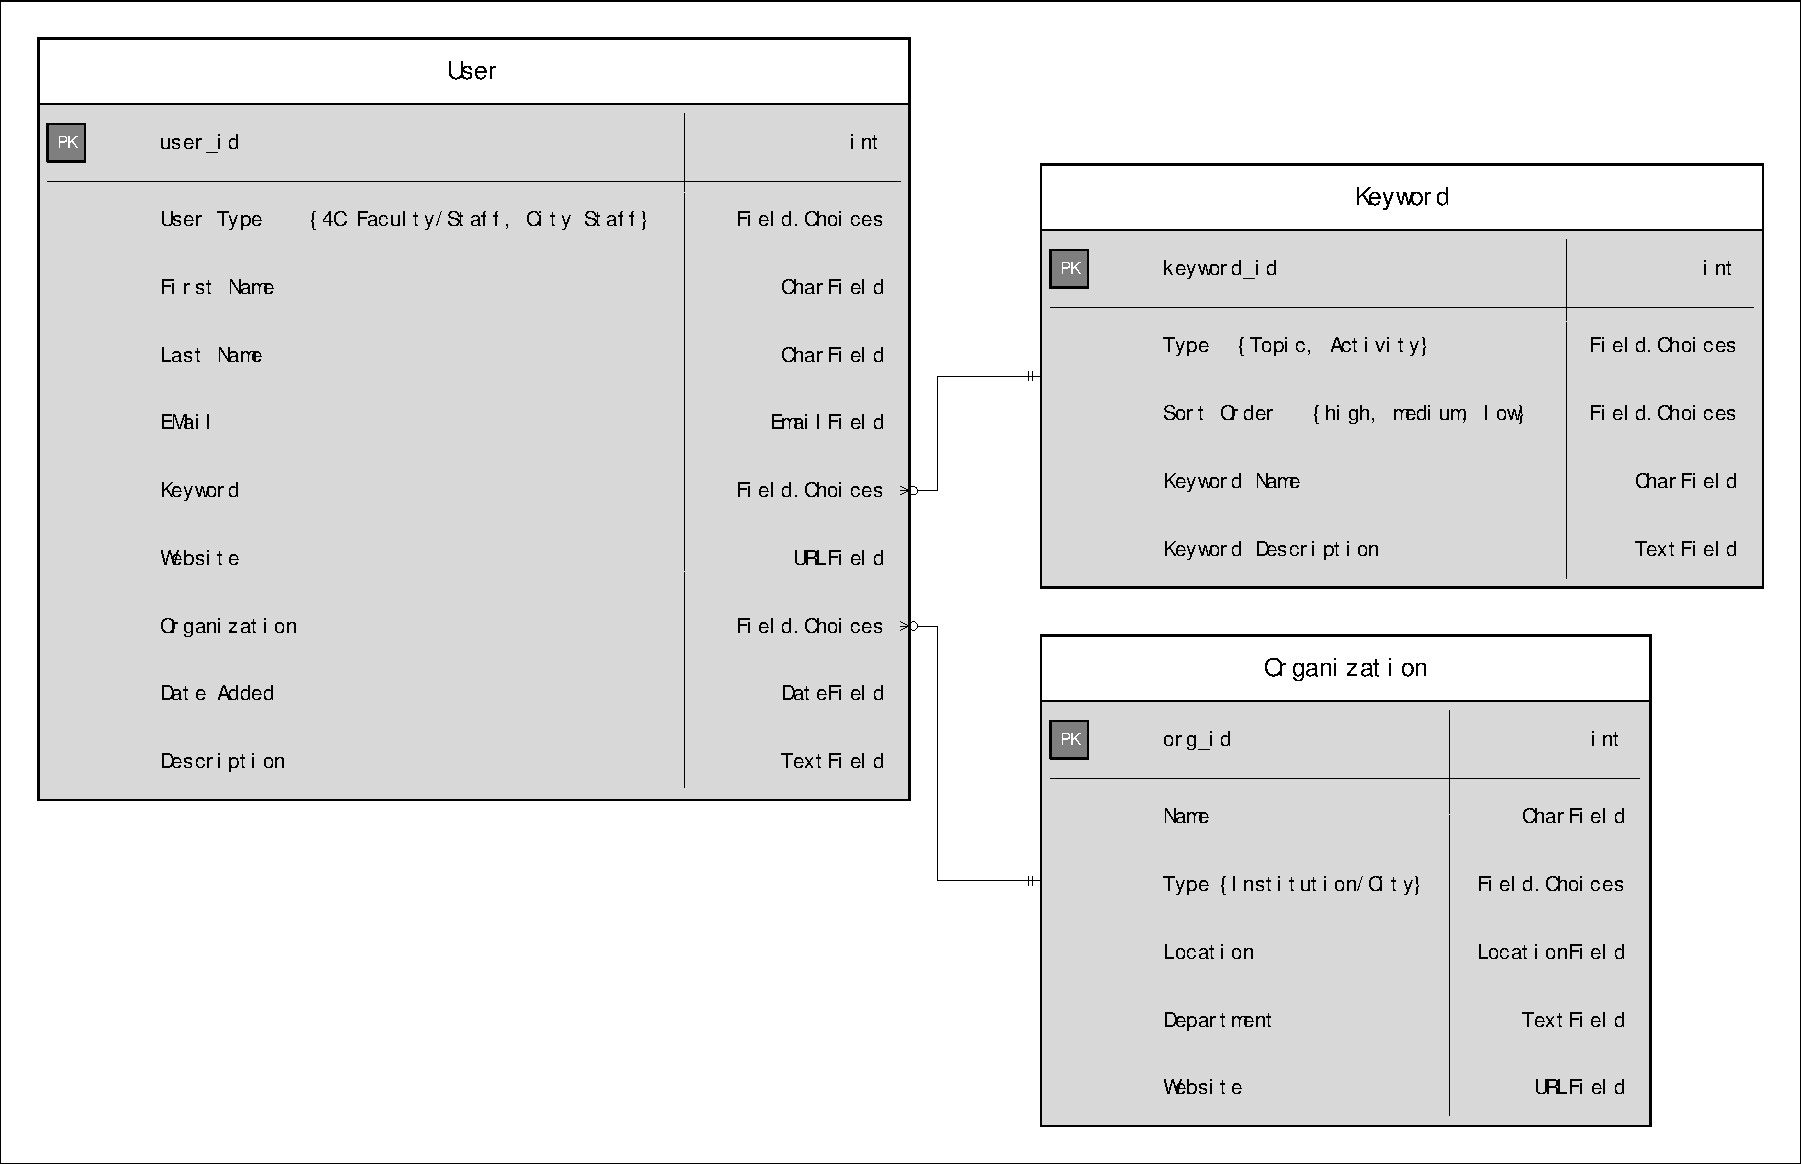
\includegraphics[width=\textwidth,trim=4 4 4 4,clip]{database-design.pdf}
\newpage
\section{Wizard Data Flow}
\label{sec:wizardDataFlow}
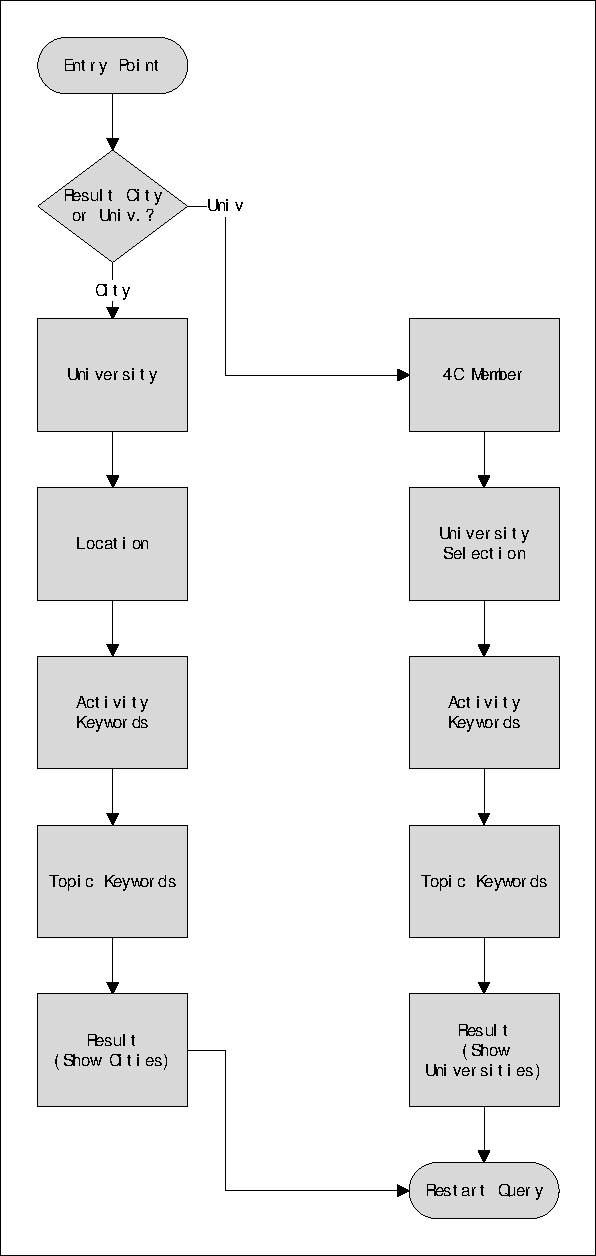
\includegraphics[width=\textwidth,trim=4 4 4 4,clip,height=8in,keepaspectratio]{wizard-data-flow.pdf}
\newpage
\section{Data display}
\label{sec:dataDisplay}
Data will be displayed in a tabular format for both organizations and people.
For the organizations view, the name of the organization POC will be displayed
along with the organization name, and department. A button will be displayed to
show extended information about the organization.
\par For the person view, the person's name will be displayed along with their
department or university. The email address of the person will be displayed.
A button will appear to view extended information about the person including,
but not limited to their website, bio, and tags.
\section{API Endpoints}
\label{sec:apiEndpoints}
The Django web framework will expose an API so that other services can query all
of the keywords (all the keywords, or by keyword type). The API will also have a
view for showing all the location regions, and possible departments. It will
also allow for viewing of all organizations, and similar to keywords, the user
will be able to pick from the types of organizations.\\
For example, the endpoint my be:\\
\begin{itemize}
   \item \url{<<URL>>/api/getLocations/<<locationType>>}
   \item \url{<<URL>>/api/getKeywords/<<keywordType>>}
\end{itemize}
\end{document}
 